\begin{figure}[htbp]
  \centering
  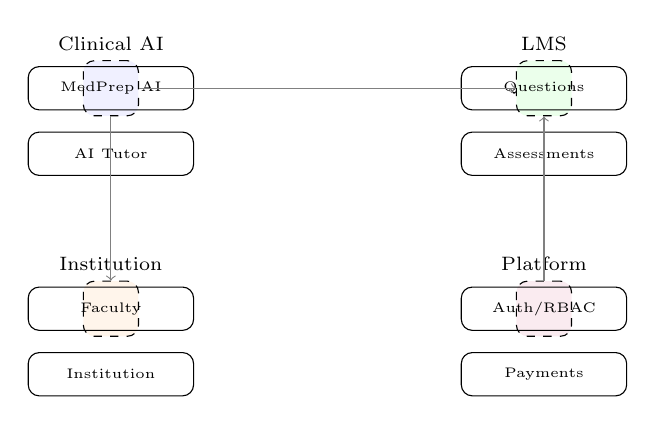
\begin{tikzpicture}[
    mod/.style={rectangle, draw, rounded corners, minimum width=2.1cm, minimum height=0.55cm, font=\tiny, align=center},
    grp/.style={rectangle, draw, dashed, rounded corners, inner sep=0.35cm}
  ]
    \node[grp, fill=blue!6, label={[font=\scriptsize]above:Clinical AI}] (g1) at (0,0) {};
    \node[mod] at (g1) {MedPrep AI};
    \node[mod, below=0.55cm] at (g1) {AI Tutor};
    \node[grp, fill=green!8, label={[font=\scriptsize]above:LMS}] (g2) at (5.5,0) {};
    \node[mod] at (g2) {Questions};
    \node[mod, below=0.55cm] at (g2) {Assessments};
    \node[grp, fill=orange!8, label={[font=\scriptsize]above:Institution}] (g3) at (0,-2.8) {};
    \node[mod] at (g3) {Faculty};
    \node[mod, below=0.55cm] at (g3) {Institution};
    \node[grp, fill=purple!8, label={[font=\scriptsize]above:Platform}] (g4) at (5.5,-2.8) {};
    \node[mod] at (g4) {Auth/RBAC};
    \node[mod, below=0.55cm] at (g4) {Payments};
    \draw[->, gray] (g1) -- (g2);
    \draw[->, gray] (g1) -- (g3);
    \draw[->, gray] (g4) -- (g2);
  \end{tikzpicture}
  \caption{NestJS module groups in MedPrepAI backend (logical layering).}
  \label{fig:module-groups}
\end{figure}
